% !TEX options=--shell-escape

% Comments start with % (percent) character and last till the end of the line.
%
% The line below tells TeXworks editor to use pdflatex for compilation
% of this document; remove it if you want to use another engine 
%
% !TEX program = pdflatex
%
% LaTeX2e document starts with \documentclass[options]{<class-name>}
% <class-name> can be one of the standard LaTeX document classes: 
% article, report or book, or some other specialised class.
%
\documentclass[a4paper,10pt]{article}
%{}
% Preamble of LaTeX document is everything before \begin{document}.
% Preamble is used to load extension packages and to set up global 
% parameters and configuration for the entire document.
%
% Extension packages providing additional functionality
\usepackage{amsmath}       % additional math environments
\usepackage{graphicx}      % graphics import from external files 
\usepackage{epstopdf}      % automates .eps to .pdf conversion 
% epstopdf package may require --shell-escape option to pdflatex
\usepackage{booktabs}      % table typesetting additions
%\usepackage{siunitx}       % number and units formatting
\usepackage{caption}       % customisation of captions
\usepackage{url}           % format url addresses
%To use this package we need to install python, pygments and have the '--shell-escape' 
\usepackage{shellesc}
\usepackage{minted}
\usepackage{listings}
%\usepackage{tikz,pgfplots} % diagrams and data plots
%
% set up caption options

% Setup the margins
\usepackage[margin=2.5cm]{geometry}

\captionsetup{format=hang,width=0.85\textwidth,labelfont=bf}

% global options for siunitx
%\sisetup{seperr,repeatunits=false,per=frac}
%
% some handy commands for referencing;
% the optional argument overrides the default label, e.g.
% \figref[FIG.~]{fig:label}
\newcommand{\figref}[2][\figurename~]{#1\ref{#2}}
\newcommand{\tabref}[2][\tablename~]{#1\ref{#2}}
\newcommand{\secref}[2][Section~]{#1\ref{#2}}

\usepackage{etoolbox}
\AtBeginEnvironment{minted}{\fontsize{10}{10}}
\AtBeginEnvironment{lstlisting}{\fontsize{10}{10}}

\lstset{language=XML, breaklines=true,
			basicstyle=\ttfamily,
           keywordstyle=\color{blue}\ttfamily,
           stringstyle=\color{red}\ttfamily,
           commentstyle=\color{green}\ttfamily
           }

% The document content starts with \begin{document} 
% and is finished with \end{document}
%
\begin{document}

\title{Parametor\\User Manual} % fill in the title here
\author{Sam Morrell}% fill in your name here
\date{September 2013\\alpha 2} % date of the report
\maketitle % formats the title section

\tableofcontents
\newpage

\section{Introduction}
Firstly, thank for you using the TORUS radiative transfer code. There's been a massive effort here in the astrophysics group to get it ready for a public release and I know that, even though I haven't personally been involved, everyone involved with the project has put in a lot of work. \\
Secondly, a little housekeeping. Please make sure that you keep your parameters files backed up before using them with Parametor. I've gone to great lengths to make sure that there's no problems with Parametor, but its still in its infancy so not all of the bugs have been ironed out of it just yet. Now that's out of the way, on with the show!\\
Who am I? I'm a third year masters student who has been working with Torus. I wrote Parametor initally as a tool for myself to help speed up my turnaround of Torus runs by helping make editing parameters files a less arduous task. My only hope this app makes your use of Torus a little bit easier, after all its a really complex and fully featured code and some of the parameters files can get a little overwhelming. If you have any feedback about Parametor, just email me at safm201@ex.ac.uk and let me know.


\section{User Interface Basics}
Upon first opening Parametor you'll see something like \figref{fig:basic-general-screen}. This is the main window of Parametor. From this window you can change all of the basic settings of your Torus parameters files. To make the process easier, the UI is split up into tabs, each with a subset of parameters that pertain to a particular part of Torus' operation. I won't go into detail about various parameters and their effect on the simulation here as there is a complete description of the parameters available in Torus' manual. Here's a brief description of each tab.

\subsection{General}
In the general tab you can alter some of the basic operating parameters of Torus. From here you can setup how Torus will input or output the currently grid to and from files, set some basic general physical parameters of the simulation such as photon count, distance and  grid size as well as controlling grid refinement. From here you can also toggle the setting that will tell Torus whether to output images and Spectral Energy Distributions (SEDs) of the loaded grid.\\
This is also where you tell Parametor which executable to use when running Torus. When opening a file, Parametor will search for a Torus executable in the current directory and use that. However, you can also choose your own by clicking the \textbf{Select} button next to the text field and choosing the executable using the open file dialog. If Parametor is enabled with an internal build of Torus, which will be discussed later on, you can leave this field completely blank. The checkbox below will tell Parametor to send the output of Torus to \textbf{torus.log} inside the working directory.

\subsection{Geometry}
In the geometry tab you can choose the geometry of the grid you're going to be using, as well as adjusting the parameters associated with the geometry. The fields visible in this form will depend on the selected geometry. To select the geometry to be used in the parameters file, simply choose it from the available ones down the left of the form. There are some geometries pre-compiled into Parametor, however you can add your own. This will be covered later on in the manual.

\subsection{Sources}
In the sources tab you can define the sources of energy in the radiative transfer simulations. From this tab you can add and remove sources as well as adjusting your sources' physical parameters such as position, mass, radius and effective temperature; as well as the continuum of their spectra.
To get started, add a source using the \textbf{Add Source} button below the list. When you select the source, the fields on the left will be populated with the appropriate data. When you're done editing the source to your liking, simply click the \textbf{Apply} button to apply your changes. Unwanted sources can be removed by selecting them and clicking the \textbf{Remove Source} button.

\subsection{Dust}
In the dust tab you can manage and adjust the properties of the dust populations within your simulation. To enable this tab, toggle the 'Dust Physics' checkbox in the  \textbf{General} tab. From here you can add and remove dust populations as well as adjust the physical properties of each such grain type and grain size. To add a dust population simply click the \textbf{Add Population} button. When you select a population from the list, the fields will be populated with the appropriate data. When you've finished editing the population simply click the \textbf{Apply} button to apply your changes. You can remove a population by selecting it from the list and clicking the \textbf{Remove Population} button.

\subsection{SED}
In this SED section you can manage the properties of the outputted Spectral Energy Distributions (SEDs). To enable this tab, go to the \textbf{General} tab and toggle the \textbf{Spectrum} checkbox. This tab allows you to adjust the settings of your SEDs such as wavelength range and units. Below each list of angles you'll see a \textbf{Generate} button. This will bring up a window that will allow you to quickly and easily populate the corresponding list with regularly spaced angles. Simply provide a minimum angle, maximum angle and number of inclinations and Parametor will do the rest. These angles can either be linearly spaced or cos spaced.

\subsection{Image}
In the image section you can manage the images Torus will output, as well as easily adjust their properties. From here you can adjust properties such as the image size, resolution and position with respect to the grid. To add an image simply click the \textbf{Add Image} button. To alter any of the image properties simply select the image from the list and the fields on the right will be populated with the appripriate data. When you're done editing simply click the  \textbf{Apply} button to apply your changes. An image can be easily removed by selecting it from the list and clicking the \textbf{Remove Image} button. 

\begin{figure}
\centering
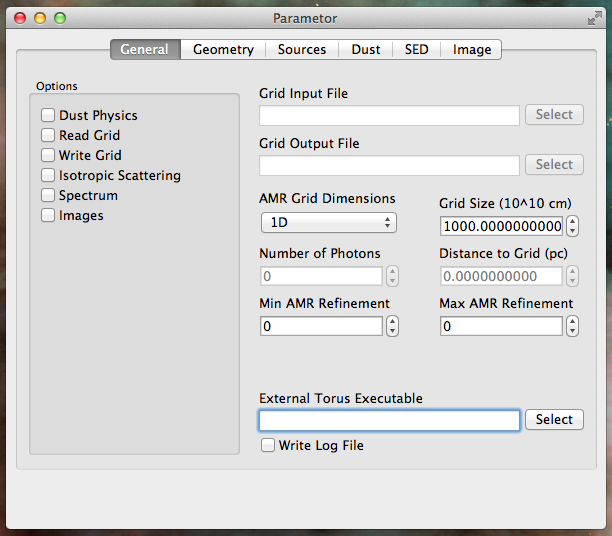
\includegraphics[width=12.5cm]{img/basics-general.png}
\caption{The main window of Parametor. The tabs along the top will show different subsets of the parameters, sorted into logical groupings.}
\label{fig:basic-general-screen}
\end{figure}

\section{Compiling Torus}
Before you can start using Torus, you first need to compile on it. This can be quite a daunting task, however Parametor can automate this for you. To compile Torus using Parametor you'll need to have \textbf{tar}, \textbf{gcc} and \textbf{gfortran} installed on your system. If you're using a Mac this can be easily done by installing Xcode (free from the App Store) and installing \textbf{Command Line Tools} from the Downloads section of the preferences. You may need to run the command below to make sure that you're using the correct installation of Xcode before you can run \textbf{make}.

\begin{verbatim}
	sudo xcode-select -switch /Applications/Xcode.app/Contents/Developer
\end{verbatim}

Next you can open up Parametor, goto the \textbf{Run} menu and select \textbf{Update Torus from Source}. This will open up a window like the one shown in \figref{fig:update-from-source}. Firstly, you choose a directory (preferably empty) that the torus source can be extracted to and built in. Just click the select button next to the 'Torus Build Directory' box to choose a directory from a file picker. Next you'll need to obtain a source tarball of Torus. This can be obtained from		 the website. You can choose it in the same way as the build directory. If you wish to have FITS file support in Torus, you'll need to download and compile the \textbf{cfitsio} library, toggle the 'Use FITS File Support' checkbox and make sure you select the library directory (if required) in the appropriate text box. The other build flags allow you switch OpenMP and MPI on and off. Choose the ones appropriate for your needs. The advanced options allow you to change the command that's executed in the make stage, if the command on your system is different. The additional commands textbox is there in case it's needed and any flags entered into this box are passed into the build. Finally, the 'Update Internal Torus Build' is an important one, I'll go into that in the next section. When all of these settings are configured as you'd like them, click the \textbf{Compile Torus} button and Parametor will do the rest.

\subsection{Internal Builds of Torus}
The traditional way to run Torus on a parameters file is to either copy the executable into the working directory or create a symbolic link and then run Torus from a terminal window. Parametor now allows Torus to be run much more easily by defining an executable anywhere on the system to be used as the executable. However, you can also allow Torus to copy a version of Torus inside the App bundle  or Application directory, meaning that you don't even need to worry about setting the executable and Parametor will perform all runs with its own internal build. You can bundle a new build of Torus by selecting the  \textbf{Update Internal Build} checkbox while updating or you can provide a pre-compiled executable by choosing \textbf{Run $>$ Update Torus from Executable} and choosing the executable file from the open file dialog.

\begin{figure}
\centering
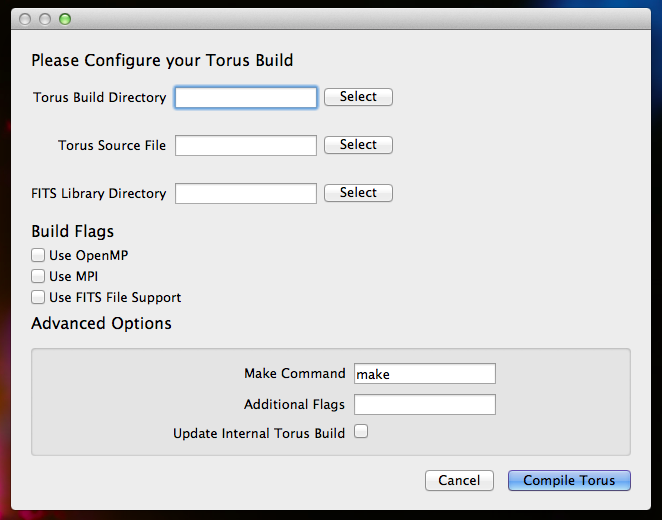
\includegraphics[width=12.5cm]{img/update-from-source.png}
\caption{This is the Update from Source window. This is how you configure Torus for compilation from within Parametor.}
\label{fig:update-from-source}
\end{figure}

\section{Running Torus}
It's possible to run torus on the open parameters file in one of two ways. You can either run torus from an executable that you define, which can be done by selecting it from the \textbf{External Torus Executable} setting in the General tab, or Parametor can run its internal build of Torus. When Torus is compiled using the built in dialog, you can tell Parametor to Update its internal build. This will copy the compiled executable inside the app and allow it to run wherever its needed. If you leave the external torus executable field blank, Torus will run the internal build. The outputs of Torus will be saved in the same directory as the parameters file, just as with a normal build.

To run Torus on your parameters file simply open it in Parametor, either by opening it from the file menu or by dragging the file onto the app, and go to \textbf{Run} $>$ \textbf{Run Torus}. This will open up the Torus Console (shown in \figref{fig:run-torus-console}) and display the progress of the run. You can cancel it at any time by closing the window or pressing the \textbf{Quit Torus} button.

\begin{figure}
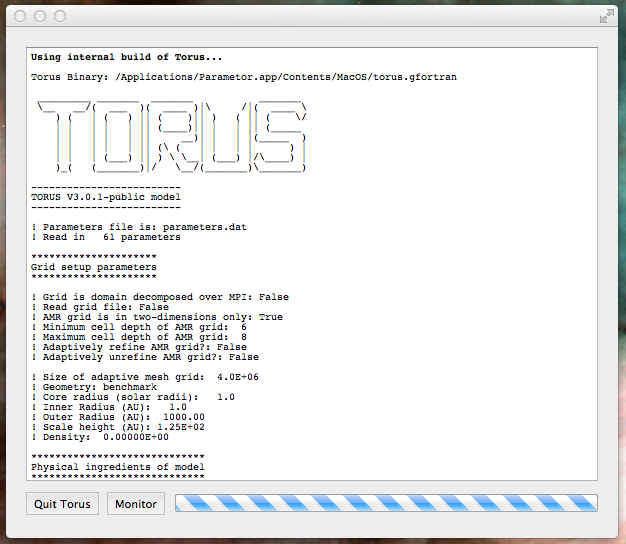
\includegraphics[width=12.5cm]{img/run-torus-console.png}
\caption{This shows the Torus Console, which is used to run Torus using the currently open parameters file.}
\label{fig:run-torus-console}
\end{figure}

\subsection{While Torus is Running}
\figref{fig:run-torus-console} shows the execution window for the current Torus session. This window shows the command line output of Torus while it's running. The \textbf{Monitor} button will show the Torus Runtime Monitor for the current session, giving in depth information of the currently running session. The progress bar at the bottom of the window gives an indication of the progress through your current run. Since it's very difficult to predict the progress while torus is setting up the grid, the progress bar remains indeterminate until SEDs and images are being calculated.

\subsection{Monitoring Torus at Runtime}
While the Torus Console is open you can press the \textbf{Monitor} button to monitor Torus while it's running. This window gives you information about the state of execution of the current Torus session. From here you can see the amount of time the current session has been running as well as a breakdown of the events that have happened during that time. If the Lucy algorithm is being used for the current run, a graph of the convergence is available in the \textbf{Convergence} tab.

\section{Tools}

\subsection{SED Viewer}
Parametor includes tools for basic SED visualisation. To open the window, simply goto \textbf{Analyse $>$ SED Viewer} and with will open the SED Viewer window; which can be seen in \figref{fig:analyse-sed-viewer}. To the left of the window you will see a list of all the files in the current directory that Parametor believes it can visualise. To display one, simply click on it. Parametor will then plot it on the graph. SED data output by torus has 5 components, stellar direct, stellar scattered, thermal direct, thermal scattered and a combined plot of the other 4. By default Parametor will visualise all of these, however you can easily toggle each component on or off using the checkboxes beneath the plot. You can identify each line using the legend above the plot.

\begin{figure}
\centering
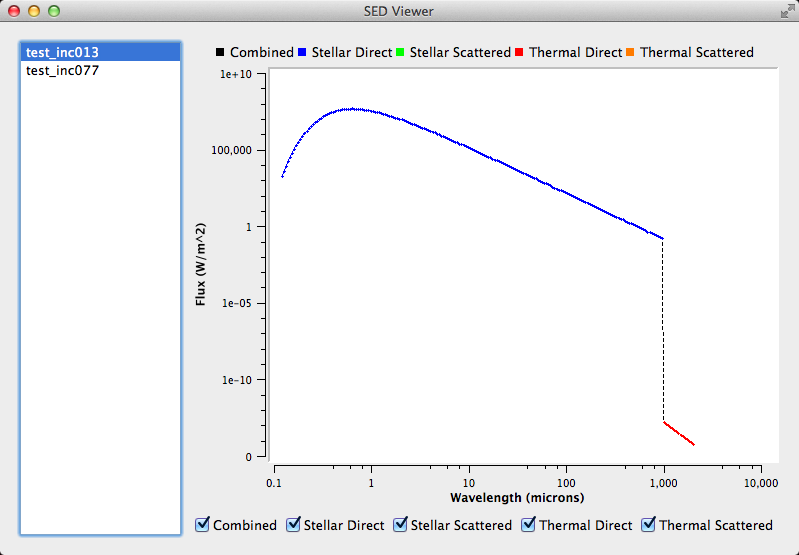
\includegraphics[width=12.5cm]{img/analyse-sed-viewer.png}
\caption{The SED viewer built into Parametor allows you to quickly and easily visualise the data output by Torus.}
\label{fig:analyse-sed-viewer}
\end{figure}

\subsection{Unit Converter}
It can often by difficult for a physicist when working with different units. As astrophysics has so many different units, I decided to build a units converter in to Parametor; seen in \figref{fig:tool-unit-converter}. It can currently convert both distances and wavelengths. The appropriate unit type can be selected from the tabs along the top of the window. To convert simply select a source unit and type the value in on the left, then select an output unit and press the \textbf{Convert} button. This will populate the output field with the appropriate value. If there are any more units that would be useful included in here then just email me and let me know.

\begin{figure}
\centering
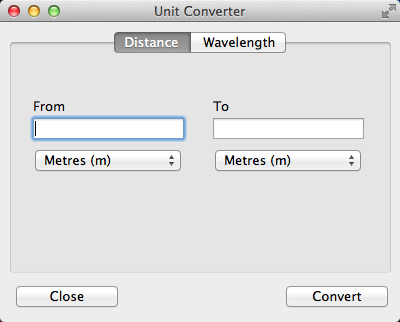
\includegraphics[width=12.5cm]{img/tool-unit-converter.png}
\caption{This screenshot shows the unit converter tool, built into Parametor.}
\label{fig:tool-unit-converter}
\end{figure}

\section{Advanced Topics}

\subsection{Defining Custom Parameters}
Parametor contains a specification for all parameters supported in the manual at the time of writing, which means that everything in your parameters files should trickle through. They are compiled into the app inside \textbf{torus-input-definitions.xml}. In an attempt to be flexible as well as remaining easy to use, Parametor allows the default parameter specification to be overridden or added to on an item by item basis. You can do this by writing the alterations into a file titled \textbf{torus-input-definitions.xml} which is placed into the same directory as the Parametor binary (inside the \textbf{Parametor.app/Contents/MacOS} directory on a Mac). The file is set out like so. First we have a root \textbf{\textit{parameters}} tag that contains the whole specification. Next, each subset of parameters is split into groups, defined by a \textbf{\textit{group}} tag. Inside each of these group tags there's a list of parameters, defined by self-closing \textbf{\textit{input}} tags, with the properties of each parameters provided by the tags' attributes. The attributes for each property are...
\begin{list}{-}
\item \textbf{name}: The name attribute tells Parametor the name of the parameter.
\item \textbf{default}: This provides Parametor with the default value of the parameter, in case it is required and undefined.
\item \textbf{canGroup}: Tells Parametor whether it can group this property together if multiple items have the same value for the property. I.E. All images share the same number of pixels, so it can be represented as a single parameter, rather than independently defined for each image. The allowed values for this property are 'yes' and 'no'.
\item \textbf{type}: Tells Parametor what data type the parameter is expecting to be. The available types are 'bool', 'string', 'int' and 'double'.
\item \textbf{isRequired}: Tells Parametor whether it needs to include this parameter in the parameters file regardless of whether it was previously defined in the parameters or defined by the user. Also, allows easy first time setup of a parameters file by adding all the parameters you need to run out of the box.
\end{list}

A basic file would look something like this...

\
\begin{lstlisting}
<?xml version="1.0" encoding="utf-8"?>
<parameters>
    <group name="misc">
        <input name='maxmemory' default='240000' canGroup='no' type='int' isRequired='true'/>
    </group>
</parameters>
\end{lstlisting}

\subsection{Defining Custom Geometries}
Parametor comes pre-compiled with the geometries officially supported in the public release. They are compiled into the Parametor executable in the \textbf{geometries.xml} file. Just as the parameter speficication, geometires can be added or modified by placing your own \textbf{geometries.xml} file in the same directory as the Parametor executable. The exceptions are that the room tag is \textbf{geometries}. Each grouping of parameters completely defines a geometry. These are enclosed inside \textbf{geometry} tags, which are named using the \textbf{name} attribute. This is the text the geometry parameter will have in order to use the geometry, as well as being the text that will show up in the list box down the side of geometries tab.
\\
The specification for the \textbf{shakara} geometry looks something like this, which should give you a good starting place for defining your own.
\begin{lstlisting}
<geometries>
        <geometry name="shakara" >
                <input name='mdisc' default='1' canGroup='no' type='double' isRequired='true' label="Disk Mass (Solar Mass)" />
                <input name='alphadisc' default='1' canGroup='no' type='double' isRequired='true' label="Disc Density"/>
                <input name='betadisc' default='1' canGroup='no' type='double' isRequired='true' label="Disc Scaleheight"/>
                <input name='rinner' default='1' canGroup='no' type='double' isRequired='true' label="Inner Disc Radius"/>
                <input name='router' default='1' canGroup='no' type='double' isRequired='true' label="Outer Disc Radius"/>
                <input name='height' default='1' canGroup='no' type='double' isRequired='true' label="Disc Scaleheight at 100 AU"/>
                <input name='rgapinner' default='1' canGroup='no' type='double' isRequired='true' label="Inner Radius of Gap"/>
                <input name='rgapouter' default='1' canGroup='no' type='double' isRequired='true' label="Outer Radius of Gap"/>
                <input name='rhogap' default='1' canGroup='no' type='double' isRequired='true' label="Minimum Gap Density (g / cm3)"/>
                <input name='smoothinneredge' default='true' canGroup='no' type='bool' isRequired='true' label="Inner Edge Exponential Density Decay"/>
                <input name='dusttogas' default='0.01' canGroup='no' type='double' isRequired='true' label='Dust to Gas Ratio' />
	</geometry>
</geometries>
\end{lstlisting}


\section{Links}
This section is where you can find some useful links:

\begin{list}{-}{}
\item The Torus Homepage:\\
\url{http://www.astro.ex.ac.uk/people/th2/torus_html/homepage.html}

\end{list}

\pagebreak

\section{Appendices}

\subsection{Appendix A: Torus Input Specification Code Listing (torus-input-specification.xml)}

\begin{lstlisting}
<?xml version="1.0" encoding="utf-8"?>
<parameters>
    <group name="misc">
        <input name='maxmemory' default='240000' canGroup='no' type='int' isRequired='true'/>
        <input name='outputfile' default='' canGroup='no' type='string' isRequired='false'/>
        <input name='inputfile' default='' canGroup='no' type='string' isRequired='false'/>
        <input name='readgrid' default='false' canGroup='no' type='bool' isRequired='true'/>
        <input name='writegrid' default='false' canGroup='no' type='bool' isRequired='true'/>
        <input name='justdump' default='false' canGroup='no' type='bool'/>
        <input name='amr1d' default='false' canGroup='no' type='bool' isRequired='true'/>
        <input name='amr2d' default='false' canGroup='no' type='bool' isRequired='true'/>
        <input name='amr3d' default='false' canGroup='no' type='bool' isRequired='true'/>
        <input name='dorefine' default='true' canGroup='no' type='bool' isRequired='true'/>
        <input name='dounrefine' default='true' canGroup='no' type='bool' isRequired='true'/>
        <input name='mindepthamr' default='5' canGroup='no' type='int' isRequired='true'/>
        <input name='maxdepthamr' default='31' canGroup='no' type='int' isRequired='true'/>
        <input name='amrgridsize' default='1000' canGroup='no' type='double' isRequired='true'/>
        <input name='griddistancescale' default='1.d10' canGroup='no' type='double' isRequired='false'/>
        <input name='cylindrical' default='false' canGroup='no' type='bool'/>
        <input name='geometry' default='sphere' canGroup='no' type='string' isRequired='true'/>
        <input name='splitovermpi' default='false' canGroup='no' type='bool' isRequired='true'/>
        <input name='binaryxml' default='true' canGroup='no' type='bool'/>
        <input name='refineonmass' default='false' canGroup='no' type='bool'/>
        <input name='refineontemperature' default='false' canGroup='no' type='bool'/>
        <input name='refineonionization' default='false' canGroup='no' type='bool'/>
        <input name='dophotorefine' default='false' canGroup='no' type='bool'/>
        <input name='amrtolerance' default='1.d-3' canGroup='no' type='double'/>
        <input name='amrtemperaturetol' default='1.d-3' canGroup='no' type='double'/>
        <input name='amrspeedtol' default='1.d-3' canGroup='no' type='double'/>
        <input name='amrionfractol' default='1.d-3' canGroup='no' type='double'/>
        <input name='amrrhoetol' default='1.d-3' canGroup='no' type='double'/>
        <input name='masstol' default='1.d-5' canGroup='no' type='double'/>
        <input name='timeunit' default='1.d0' canGroup='no' type='double'/>
        <input name='lengthunit' default='1.d0' canGroup='no' type='double'/>
        <input name='massunit' default='1.d0' canGroup='no' type='double'/>
        <input name='radeq' default='false' canGroup='no' type='bool' isRequired="true"/>
        <input name='nphotons' default='1000' canGroup='no' type='int' isRequired="true"/>
    </group>

    <group name="source">
        <input name='nsource' default='1' canGroup='no' type='int' isRequired='true'/>
        <input name='pointsource' default='false' canGroup='yes' type='bool' isRequired='true'/>
        <input name='radius' default='1.d0' canGroup='yes' type='double' isRequired='true'/>
        <input name='teff' default='1.d0' canGroup='yes' type='double' isRequired='true'/>
        <input name='mass' default='1.d0' canGroup='yes' type='double' isRequired='true'/>
        <input name='contflux' default='none' canGroup='yes' type='string' isRequired='true'/>
        <input name='sourcepos' default='0.d0,0.d0,0.d0' canGroup='yes' type='string' isRequired='true'/>
        <input name='velocity' default='0.d0,0.d0,0.d0' canGroup='yes' type='string' isRequired='false'/>
        <input name='probsource' default='0.d0' canGroup='no' type='string'/>
    </group>

    <group name="dust">
        <input name='dustphysics' default='true' canGroup='no' type='bool' isRequired='true'/>
        <input name='iso_scatter' default='true' canGroup='no' type='bool' isRequired='true'/>
        <input name='graintype' default='sil_dl' canGroup='no' type='string' isRequired='true'/>
        <input name='grainFrac' default='1' canGroup='no' type='double' isRequired='true'/>
        <input name='amin' default='0.12' canGroup='no' type='double' isRequired='true'/>
        <input name='amax' default='0.1201' canGroup='no' type='double' isRequired='true'/>
        <input name='qdist' default='0.01' canGroup='no' type='double' isRequired='true'/>
    </group>

    <group name="hydro">
        <input name='radiationHydrodynamics' default='false' canGroup='no' type='bool' isRequired='true'/>
    </group>

    <group name="sed">
        <input name='ninc' default='0' canGroup='no' type='int' isRequired='true'/>
        <input name='inclinations' default='' canGroup='no' type='string' isRequired='false'/>
        <input name='posangs' default='' canGroup='no' type='string' isRequired='false'/>
        <input name='firstinc' default='' canGroup='no' type='int' isRequired='false'/>
        <input name='lastinc' default='' canGroup='no' type='int' isRequired='false'/>
        <input name='firstPA' default='' canGroup='no' type='int' isRequired='false'/>
        <input name='lastPA' default='' canGroup='no' type='int' isRequired='false'/>
        <input name='sedwavlin' default='false' canGroup='no' type='bool' isRequired='true'/>
        <input name='sedcosspaced' default='false' canGroup='no' type='bool' isRequired='true'/>
        <input name='sedlammin' default='0.01' canGroup='no' type='double' isRequired='true'/>
        <input name='sedlammax' default='1000' canGroup='no' type='double' isRequired='true'/>
        <input name='sised' default='true' canGroup='no' type='bool' isRequired='true'/>
        <input name='filename' default='' canGroup='no' type='string' isRequired='true' />
    </group>

    <group name="image">
        <input name='image' default='false' canGroup='no' type='bool' isRequired='true'/>
        <input name='nphotons' default='1000' canGroup='yes' type='double'/>
        <input name='distance' default='100' canGroup='yes' type='double'/>
        <input name='imageaxisunits' default='AU' canGroup='yes' type='string'/>
        <input name='imagesize' default='whole grid' canGroup='yes' type='double'/>
        <input name='polimage' default='false' canGroup='yes' type='bool'/>
        <input name='imagefile' default='' canGroup='no' type='string' />
        <input name='lambdaimage' default='6562.8' canGroup='yes' type='int' />
        <input name='imagetype' default='' canGroup='yes' type='string' />
        <input name='npixels' default='200' canGroup='yes' type='int' />
        <input name='inclination' default='0' canGroup='yes' type='double' />
        <input name='positionangle' default='0' canGroup='yes' type='double' />
        <input name='fitsbitpix' default='-32' canGroup='yes' type='int' />
    </group>
</parameters>

\end{lstlisting}

\subsection{Appendix B: Geometry Specification Code Listing (geometries.xml)}
\begin{lstlisting}
<geometries>
        <geometry name="shakara" >
                <input name='mdisc' default='1' canGroup='no' type='double' isRequired='true' label="Disk Mass (Solar Mass)" />
                <input name='alphadisc' default='1' canGroup='no' type='double' isRequired='true' label="Disc Density"/>
                <input name='betadisc' default='1' canGroup='no' type='double' isRequired='true' label="Disc Scaleheight"/>
                <input name='rinner' default='1' canGroup='no' type='double' isRequired='true' label="Inner Disc Radius"/>
                <input name='router' default='1' canGroup='no' type='double' isRequired='true' label="Outer Disc Radius"/>
                <input name='height' default='1' canGroup='no' type='double' isRequired='true' label="Disc Scaleheight at 100 AU"/>
                <input name='rgapinner' default='1' canGroup='no' type='double' isRequired='true' label="Inner Radius of Gap"/>
                <input name='rgapouter' default='1' canGroup='no' type='double' isRequired='true' label="Outer Radius of Gap"/>
                <input name='rhogap' default='1' canGroup='no' type='double' isRequired='true' label="Minimum Gap Density (g / cm3)"/>
                <input name='smoothinneredge' default='true' canGroup='no' type='bool' isRequired='true' label="Inner Edge Exponential Density Decay"/>
                <input name='dusttogas' default='0.01' canGroup='no' type='double' isRequired='true' label='Dust to Gas Ratio' />
	</geometry>
        <geometry name="sph" label="Smooth Particle Hydro">
            <input name='sphdatafilename' default='' canGroup='no' type='string' isRequired='true' label="SPH File" />
            <input name='inputFileFormat' default='ascii' canGroup='no' type='string' isRequired='true' label="Input Format (ascii or binary)" />
            <input name='sphNormLimit' default='0.5' canGroup='no' type='double' isRequired='true' label="Normalisation Threshold" />
            <input name='kerneltype' default='0' canGroup='no' type='int' isRequired='true' label="Kernel Type" />
            <input name='useHull' default='false' canGroup='no' type='bool' isRequired='true' label="Use Hull Particle Method" />
            <input name='hcritPercentile' default='0.8' canGroup='no' type='double' isRequired='true' label="Percentile of hcrit" />
            <input name='hmaxPercentile' default='0.99' canGroup='no' type='double' isRequired='true' label="Percentile of hmax" />
            <input name='discardsinks' default='false' canGroup='no' type='bool' isRequired='true' label="Discard Sink Particles" />
        </geometry>
        <geometry name="fitsfile" >
                <input name='fitsgridfile' default='' canGroup='no' type='string' isRequired='false' label='Geometry File'/>
        </geometry>
        <geometry name="benchmark" >
                <input name='rinner' default='1' canGroup='no' type='double' isRequired='true' label='Inner Disc Radius (AU)'/>
                <input name='router' default='1000' canGroup='no' type='double' isRequired='true' label='Outer Disc Radius (AU)'/>
                <input name='height' default='100' canGroup='no' type='double' isRequired='true' label='Disc Scaleheight at 100 AU (AU)'/>
                <input name='rho' default='8.12e-16' canGroup='no' type='double' isRequired='true' label='Density at Inner Edge of Midplane'/>
        </geometry>
</geometries>

\end{lstlisting}

\end{document}
